\chapter{Exercise Solutions}

\section{1. Science skills}

\subsection{Exercise 1-1} 
\begin{multicols}{4}
\begin{enumerate}[noitemsep, label=\textbf{\arabic*}. ] 
\item %Carry out the following calculations
  \begin{enumerate}[itemsep=5pt, label=\textbf{(\alph*)} ] 
    \item $3,63 \times 10^6$
    \item $37,83$
    \item $6,3 \times 10^{−4}$
    \end{enumerate}
\item %Write the following in scientific notation using Table 1.3 as a reference.
    \begin{enumerate}[itemsep=5pt, label=\textbf{(\alph*)} ] 
    \item $5,11 \times 10^{5} \text{ V}$
    \item $1,0 \times 10^{-1} \ell$
    \item $5 \times 10^{-7} \text{ m}$
    \item $2,50 \times 10^{-7} \text{ m}$
    \item $3,5 \times 10^{-2} \text{ g}$
    \end{enumerate}
 \item %Write the following using the prefixes in Table 1.3.
    \begin{enumerate}[itemsep=5pt, label=\textbf{(\alph*)} ] 
    \item $0,1602 \text{ aC}$
    \item $1,992 \text{ MJ}$
    \item $59,8 \text{ kN}$
    \item $2,5 \text{ mA}$
    \item $7,5 \text{ km}$
    \end{enumerate}
\end{enumerate}
\end{multicols}
\subsection{Exercise 1-2} 
\begin{multicols}{3}
\begin{enumerate}[itemsep=5pt, label=\textbf{\arabic*}. ]
\item %Write the following quantities in scientific notation
    \begin{enumerate}[itemsep=5pt, label=\textbf{(\alph*)} ] 
    \item $1,01 \times 10^{4} \text{ Pa}$
    \item $9,8 \times 10^2 \text{ m} \cdot \text{s}^{−2}$
    \item $1,256 \times 10^{−6} \text{ A}$
    \end{enumerate}
\item %For each of the following symbols, write out the unit in full and write what power of 10 it represents:
    \begin{enumerate}[itemsep=5pt, label=\textbf{(\alph*)} ] 
    \item microgram and $-6$
    \item milligram and $-3$
    \item kilogram and $3$
    \item megagram and $6$
    \end{enumerate}
\item %Write each of the following in scientific notation, correct to 2 decimal places:
    \begin{enumerate}[itemsep=5pt, label=\textbf{(\alph*)} ] 
    \item $1,23 \times 10^{−6} \text{ N}$
    \item $4,17 \times 10^8 \text{ kg}$
    \item $2,47 \times 10^5 \text{ A}$
    \item $8,80 \times 10^{−4} \text{ mm}$
    \end{enumerate}
\item %For each of the following, write the measurement using the correct symbol for the prefix and the base unit:
    \begin{enumerate}[itemsep=5pt, label=\textbf{(\alph*)} ] 
    \item $1,01 \mu \text{s}$
    \item $1~000 \text{ mg}$
    \item $7,2 \text{ Mm}$
    \item $11 \text{ n} \ell $
    \end{enumerate}
\item % the concorde
$234,44 \text{ m} \cdot \text{ s}^{−1}$
\item % water bp
$373 \text{ K}$
\end{enumerate}
\end{multicols}

\section {2. Classification of matter}
% \subsection{Exercise 2-1} %p. 50-51 This is a table to be completed

\subsection{Exercise 2-2} 
\begin{multicols}{3}
\begin{enumerate}[itemsep=5pt, label=\textbf{\arabic*}. ] 
\item % fill in table
  \begin{enumerate}
   \item heterogeneous mixture
   \item homogeneous mixture
   \item pure
   \item pure
   \item heterogeneous mixture
   \item homogeneous mixture
  \end{enumerate}
\item % In each of the following cases, say whether the substance is an element, a mixture or a compound. 
  \begin{enumerate}
   \item element
   \item mixture
   \item element
   \item compound
   \item compound
  \end{enumerate}         
\end{enumerate}
\end{multicols}

\subsection{Exercise 2-3} 
\begin{multicols}{3}
\begin{enumerate}[noitemsep, label=\textbf{\arabic*}. ] 
\item %formula for calcium carbonate 
\begin{enumerate}[noitemsep, label=\textbf{(\alph*)} ] 
\item compound
\item $1:1:3$
\end{enumerate}
\item %give the name of the following substances
\begin{enumerate}[noitemsep, label=\textbf{(\alph*)} ] 
\item Potassium bromide
\item Hydrochloric acid
\item Potassium permanganate
\item Nitrogen dioxide
\item Ammonium hydroxide
\item Sodium sulphate
\item Iron (III) nitrate
\item Lead (II) sulphite
\item Copper (II) hydrogen carbonate
\end{enumerate}
\item %Give the chemical formula
\begin{enumerate}[noitemsep, label=\textbf{(\alph*)} ] 
\item $\text{KNO}_3$
\item $\text{Na}_{2}\text{O}$
\item $\text{BaSO}_4$
\item $\text{AlCl}_3$
\item $\text{Mg}_{3}\text{(PO}_4\text{)}_{2}$
\item $\text{SnBr}_2$
\item $\text{Mn}_{3}\text{P}_{2}$
\end{enumerate}
\end{enumerate}
\end{multicols}

\subsection{End of chapter exercises} 
\begin{multicols}{3} 
\begin{enumerate}[itemsep=5pt, label=\textbf{\arabic*}. ] 
 \item %MCQ
\begin{enumerate}[itemsep=6pt,label=\textbf{(\alph*)}]
\item i
\item iii
\end{enumerate}
\item %Classify each of the following
\begin{enumerate}[itemsep=6pt,label=\textbf{(\alph*)}]
\item compound
\item compound
\item heterogeneous mixture
\item solution
\item solution
\item compound
\item element
\item solution
\end{enumerate}
\item %match columns
\begin{enumerate}[itemsep=5pt,label=\textbf{(\alph*)}]
\item D  
\item A
\item E
\item B
\item C
\end{enumerate}
\item %testtube with iron and sulphur
\begin{enumerate}[itemsep=5pt,label=\textbf{(\alph*)}]
\item use a magnet
\item magnetism
\end{enumerate}
\item %given descriptions
\begin{enumerate}[itemsep=5pt,label=\textbf{(\alph*)}]
 \item $\text{Ag}$
 \item $\text{KBr}$
 \item $\text{CO}_{2}$
\end{enumerate}
\item %give names
\begin{enumerate}[itemsep=5pt,label=\textbf{(\alph*)}]
 \item sodium bromide
 \item barium sulphate
 \item sulphur dioxide
 \item sulphuric acid
\end{enumerate}
\item %give formula
\begin{enumerate}[itemsep=5pt,label=\textbf{(\alph*)}]
 \item $\text{FeSO}_{4}$
 \item $\text{BF}_{3}$
 \item $\text{KMnO}_{4}$
 \item $\text{ZnCl}_{2}$
\end{enumerate}
\item %properties
\begin{enumerate}[itemsep=5pt,label=\textbf{(\alph*)}]
 \item friction
 \item durable
 \item durable
 \item shiny
 \item easily moulded
 \item fibrous
\end{enumerate}
\end{enumerate}
\end{multicols}

\section {3. States of matter and the KMT}
\subsection{End of chapter exercises} 
\begin{multicols}{3}
\begin{enumerate}[label=\textbf{\arabic*}., itemsep=5pt]
\item %give one word/term
\begin{enumerate}[label=\textbf{(\alph*)}, itemsep=7pt]
\item sublimation
\item evaporation
\end{enumerate}
\item %water
\begin{enumerate}[label=\textbf{(\alph*)}, itemsep=7pt]
\item see definition
\item liquid to gas
\end{enumerate}
\item %describe a solid
see definition
\item %table
\begin{enumerate}
 \item solid, solid, gas, solid, gas, solid
\item carbon 
\item helium
\end{enumerate}
\item %pics
\scalebox{.3}{
\begin{pspicture}(0,0)(10,2.6)
\SpecialCoor
%\psgrid[gridcolor=lightgray]

\rput(0,0.5){\psframe(0,0)(3,2)
\rput(0.1,0){\multirput(0.2,0.2)(0.4,0){7}{\pscircle(0,0){0.2}}
\multirput(0.4,0.55)(0.4,0){6}{\pscircle(0,0){0.2}}
\multirput(0.2,0.9)(0.4,0){7}{\pscircle(0,0){0.2}}}}

\rput(3.5,0.5){\psframe(0,0)(3,2)
\rput(0.2,0.2){\pscircle(0,0){0.2}}
\rput(0.6,0.3){\pscircle(0,0){0.2}}
\rput(1.2,0.3){\pscircle(0,0){0.2}}
\rput(1.7,0.2){\pscircle(0,0){0.2}}
\rput(2.3,0.3){\pscircle(0,0){0.2}}
\rput(2.8,0.2){\pscircle(0,0){0.2}}
\rput(0.3,0.9){\pscircle(0,0){0.2}}
\rput(0.8,0.7){\pscircle(0,0){0.2}}
\rput(1.5,0.8){\pscircle(0,0){0.2}}
\rput(2.0,0.8){\pscircle(0,0){0.2}}
\rput(2.5,0.7){\pscircle(0,0){0.2}}}

\rput(7,0.5){\psframe(0,0)(3,2)
\rput(2.5,0.5){\pscircle(0,0){0.2}}
\rput(2.4,1.7){\pscircle(0,0){0.2}}
\rput(1.5,1){\pscircle(0,0){0.2}}
\rput(0.7,1.7){\pscircle(0,0){0.2}}
\rput(0.3,0.3){\pscircle(0,0){0.2}}}

\uput[d](1.5,0.5){solid}
\uput[d](5,0.5){liquid}
\uput[d](8.5,0.5){gas}

\end{pspicture}}
\end{enumerate}
\end{multicols}


% \end{eocexercises}

\section {4. The atom}
\subsection{Exercise 4-1} 
\begin{multicols}{5}
\begin{enumerate}[noitemsep, label=\textbf{\arabic*}. ] 
\item D
\item A
\item C
\item E
\item B
\end{enumerate}
\end{multicols}
\subsection{Exercise 4-2}
\begin{multicols}{5}
\begin{enumerate}[noitemsep, label=\textbf{\arabic*}. ]
 \item %explain meaning
see definitions
\end{enumerate}
%  \item table
\begin{enumerate}[noitemsep, label=\textbf{\arabic*}. ]
\setcounter{enumi}{2}
 \item %standard notation
\begin{enumerate}[noitemsep, label=\textbf{\alph*}. ]
 \item $^{40}_{19}\text{K}$
\item $^{54}_{29}\text{Cu}$
\item $^{35}_{17}\text{Cl}$
\end{enumerate}
 \item %for the element
\begin{enumerate}[noitemsep, label=\textbf{\alph*}. ]
 \item $17$
\item $18$
\item $17$
\end{enumerate}
 \item %which of the following atoms
$^{15}_{7}\text{N}$
 \item %give x
\begin{enumerate}[noitemsep, label=\textbf{\alph*}. ]
 \item Ar
\item $40$
\item $15$
\end{enumerate}
 \item %complete table
\begin{enumerate}[noitemsep, label=\textbf{\alph*}. ]
 \item $Z$
\item $N, A$
\end{enumerate}
\end{enumerate}
\end{multicols}
\subsection{Exercise 4-3}
\begin{multicols}{5}
\begin{enumerate}[noitemsep, label=\textbf{\arabic*}. ]
 \item %MCQ
D
 \item %sulphur isotopes
\begin{enumerate}[noitemsep, label=\textbf{\alph*}. ]
 \item $16$
\item $32$ and $34$
\item $16$
\item $16$ and $18$
\end{enumerate}
 \item %MCQ
C
 \item %MCQ
A
\end{enumerate}
\begin{enumerate}[noitemsep, label=\textbf{\arabic*}. ]
\setcounter{enumi}{5}
 \item %boron
$10,8 \text{ u}$
 \item %magnesium
$24,3 \text{ u}$
\item %std notation
\begin{enumerate}[noitemsep, label=\textbf{\alph*}. ]
 \item $^{232}_{92}\text{U}$
\item $^{238}_{92}\text{U}$
\end{enumerate}
\item %MCQ
B
\item %sulphur isotopes
\begin{enumerate}[noitemsep, label=\textbf{\alph*}. ]
 \item $16$
\item  $33$
\item $16$
\item $17$
\end{enumerate}
\end{enumerate}
\end{multicols}
\subsection{End of chapter exercises} 
\begin{multicols}{4}
\begin{enumerate}[noitemsep, label=\textbf{\arabic*}. ] 
\item %give word
    \begin{enumerate}[noitemsep, label=\textbf{(\alph*)} ]
    \item atomic mass number
    \item electron orbital
    \end{enumerate}
\item %true/false
    \begin{enumerate}[noitemsep, label=\textbf{(\alph*)} ]
    \item false
    \item true
    \item true
    \item false
    \end{enumerate}
\item %MCQ
    \begin{enumerate}[noitemsep, label=\textbf{(\alph*)} ]
    \item B
    \item B
    \item A
    \item C
    \item B
    \end{enumerate}
\item %give std notation
    \begin{enumerate}[noitemsep, label=\textbf{(\alph*)} ]
    \item $^{5}_{4}\text{Be}$
    \item $^{12}_{6}\text{C}$
    \item $^{48}_{22}\text{Ti}$
    \item $^{19}_{9}\text{F}$
    \end{enumerate}
\item %electron configs
    \begin{enumerate}[noitemsep, label=\textbf{(\alph*)} ]
    \item $\text{[Ne]} 3\text{s}^2 3\text{p}^1$
    \item $\text{[Ne]} 3\text{s}^2 3\text{p}^3$
    \item $\text{[He]} 2\text{s}^2 2\text{p}^2$
    \item $\text{[He]} 2\text{s}^2 2\text{p}^6$
    \item $\text{[Ne]} 3\text{s}^2 3\text{p}^6$
    \end{enumerate}
\item %give protons,etc.
    \begin{enumerate}[noitemsep, label=\textbf{(\alph*)} ]
    \item $78 ; 117 ; 78$
    \item $18 ; 22 ; 18$
    \item $27 ; 32 ; 27$
    \item $3 ; 4 ; 3$
    \item $5 ; 6 ; 5$
    \end{enumerate}
\item %give x
  \begin{enumerate}[noitemsep, label=\textbf{(\alph*)} ]
  \item Rh
  \item $17$
  \item $9$
  \end{enumerate}
\item %isotopes
B
\item %copper amu
$63,62 \text{ u}$
\end{enumerate}
\end{multicols}
\section {5. The periodic table}
\subsection{Exercise 5-2} 
\begin{multicols}{5}
\begin{enumerate}[noitemsep, label=\textbf{\arabic*}. ] 
\setcounter{3}
\item %elements list
    \begin{enumerate}[noitemsep, label=\textbf{(\alph*)} ]  
    \item Li
\item Cl
\item Ne
\item Li
\item C
\item Li
\item Ca
\item Ne
\item Mg and Ca
    \end{enumerate}  
\end{enumerate}
\end{multicols}
\subsection{End of chapter exercises} 
\begin{multicols}{3}
    \begin{enumerate}[itemsep=6pt, label=\textbf{\arabic*}. ] 
\item %true false 
 \begin{enumerate}[noitemsep, label=\textbf{(\alph*)} ]
    \item false
    \item true
    \item false
    \item false
    \end{enumerate}
\item %one word/term 
 \begin{enumerate}[noitemsep, label=\textbf{(\alph*)} ]
    \item first ionisation energy
    \item period
    \item halogens
    \end{enumerate}
\item %compare elements 
 \begin{enumerate}[noitemsep, label=\textbf{(\alph*)} ] 
    \item $\text{Br} > \text{ Cl}$
    \item $\text{Cl} > \text{ Br}$ 
    \item $\text{Cl} > \text{ Br}$
    \item $\text{Br} > \text{ Cl}$
    \end{enumerate}
\item %draw graphs 
 \begin{enumerate}[noitemsep, label=\textbf{(\alph*)} ]
    \item \includegraphics[width=.2\textwidth]{photos/periodictable_eocex_graph1.png}
    \item \includegraphics[width=.2\textwidth]{photos/periodictable_eocex_graph2.png}
    \item 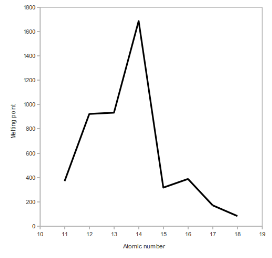
\includegraphics[width=.2\textwidth]{photos/periodictable_eocex_graph3.png}
    \item \includegraphics[width=.2\textwidth]{photos/periodic_table_eocex_graph4.png}
    \end{enumerate}
\end{enumerate}
\end{multicols}

\section {6. Chemical bonding}
\subsection{Exercise 6-1} 
\begin{multicols}{3}
\begin{enumerate}[noitemsep, label=\textbf{\arabic*}.]
\item %lewis notation
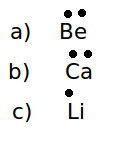
\includegraphics[width=0.1\textwidth]{photos/bonding_lewis_diagram.png}
\item %lewis molecules
\includegraphics[width=0.2\textwidth]{photos/bonding_lewis_diagram1.png}
\item %chemical reactions
\begin{enumerate}[noitemsep, label=\textbf{(\alph*)} ]
\item $\text{N: } 5$ $\text{H: } 1$ $\text{C: } 4$ $\text{H: } 1$
\item \includegraphics[width=0.1\textwidth]{photos/bonding_lewis_diagram2.png} \includegraphics[width=0.1\textwidth]{photos/bonding_lewis_diagram3.png}
\item ammonia methane
\end{enumerate}
\item %chemical compound
\begin{enumerate}[noitemsep, label=\textbf{(\alph*)} ]
\item $6$
\item $2$
\item $1$
\item $2$
\item H and O
\end{enumerate}
    \end{enumerate}
\end{multicols}
\subsection{Exercise 6-2} 
\begin{multicols}{2}
\begin{enumerate}[label=\textbf{\arabic*}.]
\setcounter{enumi}{2}
\item %simple diagrams
\begin{enumerate}[label=\textbf{\alph*}.]
 \item 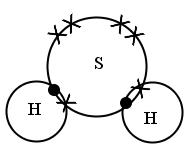
\includegraphics[width=0.2\textwidth]{photos/bonding_molecule1.png}
 \item \includegraphics[width=0.2\textwidth]{photos/bonding_molecule2.png}
\item 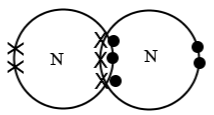
\includegraphics[width=0.2\textwidth]{photos/bonding_molecule3.png}
\item 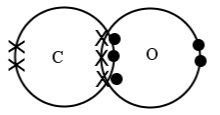
\includegraphics[width=0.2\textwidth]{photos/bonding_molecule4.png}
\end{enumerate}
\end{enumerate}
\end{multicols}
\subsection{Exercise 6-3} 

\begin{enumerate}[label=\textbf{\arabic*}.]
 \begin{multicols}{3}
\setcounter{enumi}{1}
\item %magnesium and chlorine
\begin{enumerate}[label=\textbf{\alph*}.]
 \item $1.8$
\item
\begin{enumerate}[label=\textbf{\roman*}.]
\item $\text{Mg}^{2+}$
\item $\text{Cl}^{-}$
\item $\text{MgCl}_2$
\end{enumerate}
\item $\text{Mg} + 2\text{Cl} \to \text{MgCl}_{2}$
\end{enumerate}
\end{multicols}
\item %draw lewis diagrams
\includegraphics[width=0.3\textwidth]{photos/bonding_lewis_diagrams_ion.png}
\end{enumerate}

\subsection{Exercise 6-4} 
\begin{multicols}{3}
\begin{enumerate}[label=\textbf{\arabic*}.]
\item %2 examples
\begin{enumerate}[label=\textbf{\alph*}.]
\item graphite, water
\item table salt
\item cutlery, jewellery
\end{enumerate}
\end{enumerate}
\end{multicols}
\subsection{Exercise 6-5} 
\begin{multicols}{3}
\begin{enumerate}[itemsep=6pt, label=\textbf{\arabic*}.]
\setcounter{enumi}{1}
\item %write chem formula
\begin{enumerate}[noitemsep, label=\textbf{(\alph*)} ]
\item $\text{HCN}$
\item $\text{CO}_{2}$
\item $\text{Na}_{2}\text{CO}_{3}$
\item $\text{NH}_{4}\text{OH}$
\item $\text{BaSO}_4$
\item $\text{Cu(NO}_3\text{)}_{2}$
\end{enumerate}
    \end{enumerate}
\end{multicols}

\subsection{End of chapter exercises}

\begin{enumerate}[label=\textbf{\arabic*}.]
\begin{multicols}{2}
\setcounter{enumi}{1}
\item %MCQ
B
\item %MCQ
B
\end{multicols}
\begin{multicols}{3}
\item %Lewis structures
\includegraphics[width=0.2\textwidth]{photos/bonding_morelewis.png}

\item %given lewis
\begin{enumerate}[noitemsep, label=\textbf{(\alph*)} ]
\item $1$
\item $3$
\item hydrogen and nitrogen
\end{enumerate}
\item %table
\begin{tabular}{|l|l|l|l|}\hline
 & $\text{K}^{+}$ & $\text{Ca}^{2+}$ & $\text{NH}_{4}^{+}$ \\ \hline
$\text{OH}^{-}$ & $\text{KOH}$ & $\text{Ca(OH)}_{2}$ & $\text{NH}_{4}\text{OH}$ \\ \hline
$\text{O}^{2-}$ & $\text{K}_{2}\text{O}$ & $\text{CaO}$ & $\text{(NH}_{4}\text{)}_{2}\text{O}$ \\ \hline
$\text{NO}_{3}^{-}$ & $\text{KNO}_{3}$ & $\text{Ca(NO}_{3}\text{)}_{2}$ & $\text{NH}_{4}\text{NO}_{3}$ \\ \hline
$\text{PO}_{4}^{3-}$ & $\text{K}_{3}\text{PO}_{4}$ & $\text{Ca}_{3}{(PO}_{4}\text{)}_{2}$ & $\text{(NH}_{4}\text{)}_{3}\text{PO}_{4}$ \\ \hline
\end{tabular}
\item %potassium dichromate in water
\begin{enumerate}[noitemsep, label=\textbf{(\alph*)} ]
\item potassium ($\text{K}^{+}$) dichromate ($\text{Cr}_{2}\text{O}_{7}^{2-}$)
\item $\text{K}_{2}\text{Cr}_{2}\text{O}_{7}$
\end{enumerate}
\end{multicols}
\end{enumerate}
\section {7. Transverse pulses}
\subsection{Exercise 7-1} 
\begin{multicols}{4}
\begin{enumerate}[noitemsep, label=\textbf{\arabic*}. ]
\item %pulse covers distant
$0,\dot{3} \text{ m}\cdot \text{s}^{-1}$
\item %pulse has speed
$12,5 \text{ m}$
\item %pulse has speed
$0,5 \text{ s}$
\item %how long will it take  
$80 \text{ s}$
\item %diagram shows
both move at same speed
\end{enumerate}
\end{multicols}

\subsection{Exercise 7-2} 
\begin{multicols}{4}
 \begin{enumerate}[noitemsep, label=\textbf{\arabic*}.]
\setcounter{enumi}{1}
  \item \includegraphics[height=.45\textwidth]{photos/transverse_pulses_superposition1.png}
\item 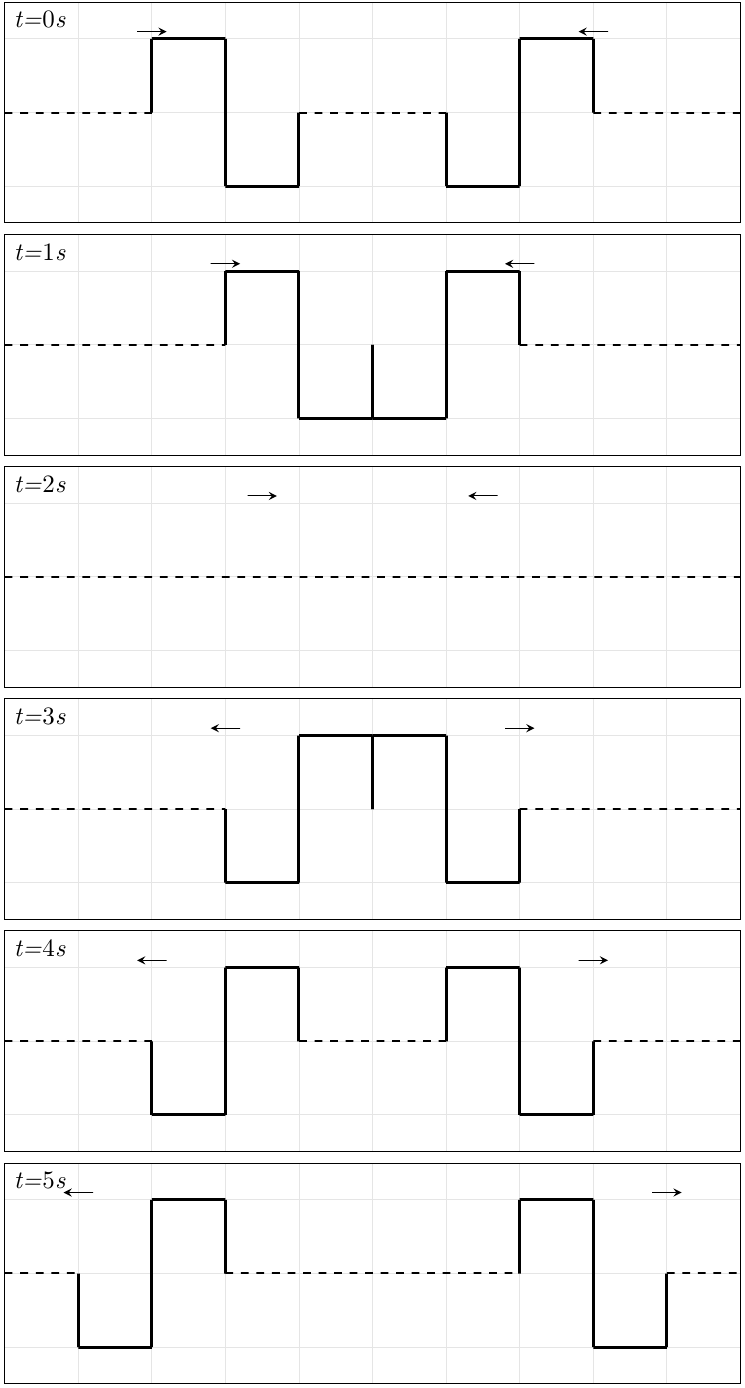
\includegraphics[height=.45\textwidth]{photos/transverse_pulses_superposition2.png}
\item \includegraphics[height=.5\textwidth]{photos/transverse_pulses_superposition.png}
\item 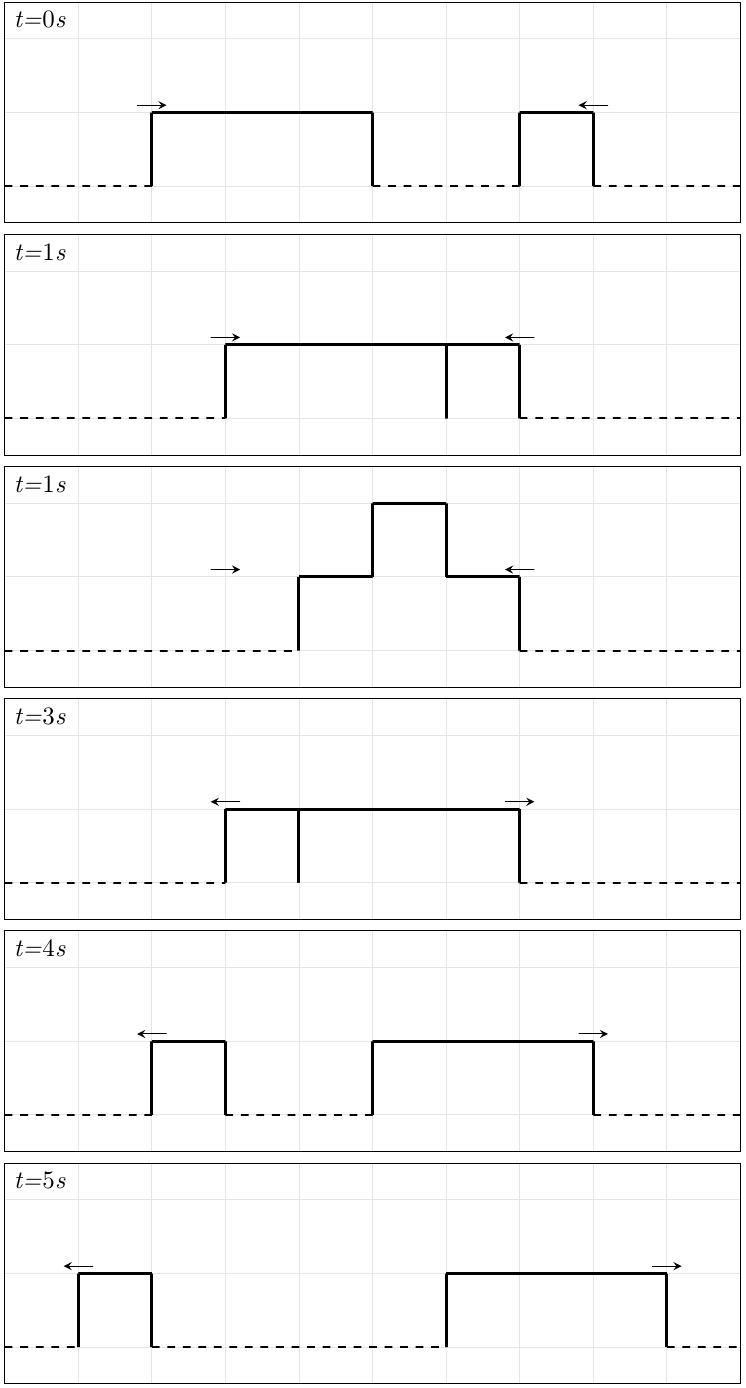
\includegraphics[height=.45\textwidth]{photos/transverse_pulses_superposition3.png}
 \end{enumerate}
\end{multicols}

\subsection{End of chapter exercises} 

\begin{enumerate}[noitemsep, label=\textbf{\arabic*}. ] 
\item %drawing
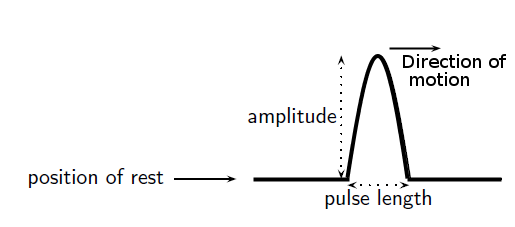
\includegraphics[width=.4\textwidth]{photos/transverse_pulses_eocex.png}
\begin{multicols}{4}
\item %pulse of speed
$15 \text{ m}$
\item %pulse covers distance
$0,3 \text{ m} \cdot \text{s}^{-1}$
\item %how long
$0,05 \text{ s}$
\end{multicols}
\end{enumerate}

\section {8. Transverse waves}
\subsection{Exercise 8-1} 
\begin{multicols}{3}
\begin{enumerate}[label=\textbf{\arabic*}.]
\item %Fill in answer
transverse
\item %transverse wave moving down
sideways
\item %answer q's about diagram
\begin{enumerate}[noitemsep,label=\textbf{\alph*}.]
\item D
\item B
\end{enumerate}
\item %draw two wavelengths
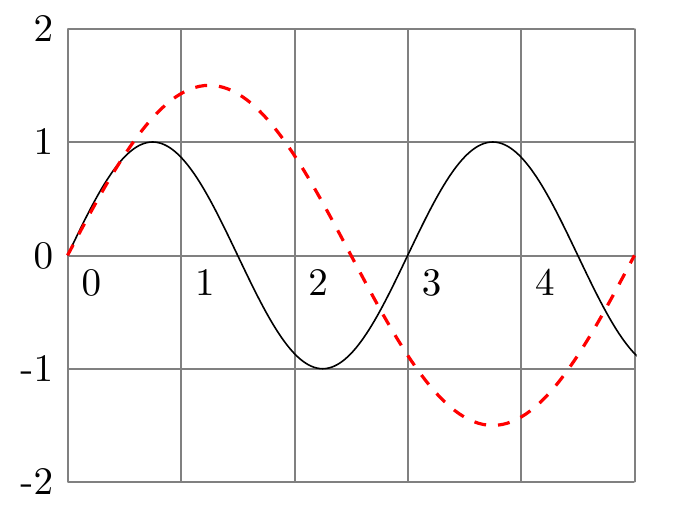
\includegraphics[width=.3\textwidth]{photos/transverse_waves_wavelengths.png}
\end{enumerate}
\begin{enumerate}[label=\textbf{\arabic*}.]
\setcounter{enumi}{5}
\item %a transverse wave
\begin{enumerate}[noitemsep,label=\textbf{\alph*}.]
\item $0,067 \text{ s}$
\item $0,075 \times 10^{-2} \text{ m}$
\end{enumerate}
\item %fly flapping wings
$0,005 \text{ s}$
\item %as the period
decrease
\item %frequency of second hand
$0,017 \text{ Hz}$
\item %microwaves
$2,99 \times 10^{8} \text{ m} \cdot \text{s}^{-1}$
\item %study diagram
\begin{enumerate}[noitemsep,label=\textbf{\alph*}.]
\item C,K
\item A,F
\item C,K
\end{enumerate}
\item %Tom is fishing
$2 \text{ m} \cdot \text{s}^{-1}$
\end{enumerate}
\end{multicols}
\subsection{End of chapter exercises} 
\begin{multicols}{4}
\begin{enumerate}[noitemsep, label=\textbf{\arabic*}. ] 
\item %a wave on a string 
 \begin{enumerate}[noitemsep, label=\textbf{(\alph*)} ]
\item $0,2 \text{ m}$
\item $1,33 \text{ s}$
\end{enumerate}
\item %water waves
 \begin{enumerate}[noitemsep, label=\textbf{(\alph*)} ]
\item $3$
\item 
\begin{enumerate}[noitemsep, label=\textbf{(\roman*)} ]
\item BD
\item AB
\item BD
\end{enumerate}
\item $0,75 \text{ m}$
\item $0,625 \text{ s}$
\item $1,60 \text{ Hz}$
\item $16,0 \text{ m} \cdot \text{s}^{-1}$
\end{enumerate}
\end{enumerate}
\end{multicols}
\section {9. Longitudinal waves}
\subsection{End of chapter exercises} 
\begin{multicols}{3}
  \begin{enumerate}[noitemsep, label=\textbf{\arabic*}.]
  \item %MCQ
A
  \item %MCQ
D
  \item %long wave taking time to pass
\begin{enumerate}[noitemsep, label=\textbf{\alph*}.]
 \item $10 \text{ m}$
\item $2 \text{ m} \cdot \text{s}^{-1}$
\end{enumerate} 
  \item %a flute
\begin{enumerate}[noitemsep, label=\textbf{\alph*}.]
 \item $-\frac{1}{256} \text{ s}$
\item $1,25 \text{ m}$
\end{enumerate}
  \end{enumerate}
\end{multicols}
\section {10. Sound}
\subsection{Exercise 10-1} 
\begin{multicols}{3}
  \begin{enumerate}[noitemsep, label=\textbf{\arabic*}. ]
  \item 
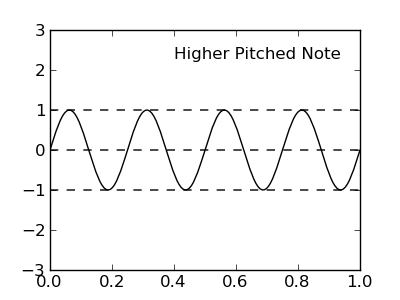
\includegraphics[width=.3\textwidth]{photos/long_waves_note1.png}
  \item 
\includegraphics[width=.3\textwidth]{photos/long_waves_note2.png}
\item
\includegraphics[width=.3\textwidth]{photos/long_waves_note3.png}
\end{enumerate}
\end{multicols}

\subsection{End of chapter exercises} 
\begin{multicols}{5}
  \begin{enumerate}[itemsep=5pt, label=\textbf{\arabic*}. ]
  \item %choose a word
    \begin{enumerate}[noitemsep, label=\textbf{(\alph*)} ]
    \item frequency
    \item amplitude
\item waveform
    \end{enumerate}
  \item %tuning fork
E
  \item %drummer
D
  \item %range of audible frequency
C
  \item %differen wave motions
C
  \item %astronauts
B
  \item %a man on cliff
E
  \item %dolphin
C
  \item %amplitude and frequency
A
  \item %jet fighter
C
    \item %sound and light
B
    \item %sound waves have fastes speed in
A
\item %two sound waves
C
\item %straw
    \begin{enumerate}[noitemsep, label=\textbf{(\alph*)} ]
    \item $340 \text{ Hz}$
    \item $680 \text{ Hz}$
    \end{enumerate}
\item %lightning storm
$1~700 \text{ m}$
\item %person yelling from 2nd floor
$0,14 \text{ s}$
\item %piece of equipment
Use earplugs
\item %what property of sound
intensity
\item %person A to person b
\item %sound can't travel in space
radios
\item %camera
$25,8 \text{ m}$
\item %mosquito
$0,57 \text{ m}$ $600 \text{ Hz}$
\item %halving frequency
increase wavelength
\item %humans
$17 \text{ mm}$
\item %elephant
$34,4 \text{ m}$
\item %ship
$1~812,5 \text{ mm}$
\item %person on cliff
$172 \text{ m}$
\item %match columns
    \begin{enumerate}[noitemsep, label=\textbf{(\alph*)} ]
    \item sound waves
    \item transverse waves
\item wavelength
\item frequency
    \item amplitude
    \item wave speed
\item wave speed
\item period
    \end{enumerate}
  \end{enumerate}
\end{multicols}

\section {11. EM radiation}
\subsection{Exercise 11-1}     
\begin{enumerate}[noitemsep, label=\textbf{\arabic*}.]
\item Infrared, visible, ultra-violet, X-rays, gamma 
\item $7,49 \times 10^{14} \text{ Hz}$
\end{enumerate}

\subsection{Exercise 11-2} 
 \begin{enumerate}[noitemsep, label=\textbf{\arabic*}. ]
  \item higher energy radiation has greater penetrating ability
\end{enumerate}

\subsection{Exercise 11-3}
\begin{multicols}{3}
  \begin{enumerate}[noitemsep, label=\textbf{\arabic*}. ]
 \item directly proportional
\item $6,6 \times 10^{-22} \text{ J}$
\item $3,3 \times 10^{-19} \text{ J}$
\end{enumerate}
\end{multicols}

\subsection{End of chapter exercises} 
\begin{multicols}{3}
\begin{enumerate}[itemsep=20pt, label=\textbf{\arabic*}.]
\item $2 \times 10^{-25} \text{ J}$
\item $3 \times 10^{-19} \text{ J}$
\item Radio, microwave, infrared, visible, ultraviolet, X-ray, gamma ray
\end{enumerate}
\end{multicols}

\section {12. The particles that substances are made of}
\subsection{End of chapter exercises} 
\begin{multicols}{3}
\begin{enumerate}[noitemsep, label=\textbf{\arabic*}. ] 
\item %give one word or term
    \begin{enumerate}[noitemsep, label=\textbf{(\alph*)} ]
  \item molecule
\item empirical formula
 \end{enumerate}
\end{enumerate}
\begin{enumerate}[noitemsep, label=\textbf{(\arabic*)} ]
\setcounter{enumi}{1}
\item %ammonia
    \begin{enumerate}[noitemsep, label=\textbf{(\alph*)} ]
 \item covalent
\item $\text{NH}_{3}$
\item 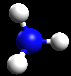
\includegraphics[width=.1\textwidth]{photos/composition_ammonia_ballstick.png}
\item \includegraphics[width=.1\textwidth]{photos/composition_ammonia_spacefill.png}
\end{enumerate}
\item %give type of molecules
    \begin{enumerate}[noitemsep, label=\textbf{(\alph*)} ]
 \item covalent molecular
\item metallic network
\item covalent network
\item covalent molecular
\item ionic network
\end{enumerate}
\item %refer to diagram
    \begin{enumerate}[noitemsep, label=\textbf{(\alph*)} ]
 \item carbon dioxide
\item $\text{CO}_2$
\item covalent
\end{enumerate}
\end{enumerate}
\end{multicols}

\section{13. Physical and chemical change}
\subsection{Exercise 13-1}
\begin{multicols}{5}
 \begin{enumerate}[noitemsep, label=\textbf{(\arabic*)} ]
  \item physical
\item chemical
\item chemical
\item physical
\item physical
 \end{enumerate}
\end{multicols}

\subsection{Exercise 13-2}
\begin{multicols}{3}
 \begin{enumerate}[noitemsep, label=\textbf{(\arabic*)} ]
  \item $68,12$
\item $136,08$
\item $246,66$
 \end{enumerate}
\end{multicols}

\subsection{End of chapter exercises}
\begin{multicols}{3}
 \begin{enumerate}[noitemsep, label=\textbf{(\arabic*)} ]
  \item 
 \begin{enumerate}[noitemsep, label=\textbf{(\alph*)} ]
\item physical change
\item chemical change
\item synthesis reaction
\end{enumerate}
\item see definitions
\item 
 \begin{enumerate}[noitemsep, label=\textbf{(\alph*)} ]
\item physical change
\item chemical change
\item chemical change
\item chemical change
\item physical change
\item physical change
\item physical change
\item chemical change
\end{enumerate}
\item
 \begin{enumerate}[noitemsep, label=\textbf{(\alph*)} ]
\item decomposition
\item synthesis
\item decomposition
\end{enumerate}
 \end{enumerate}
\end{multicols}

\section{14. Representing chemical change}
\subsection{Exercise 14-1}
 \begin{enumerate}[noitemsep, label=\textbf{(\arabic*)} ]
\begin{multicols}{5}
  \item %chem formula
 \begin{enumerate}[noitemsep, label=\textbf{(\alph*)} ]
\item $\text{FeCl}_{3}$
\item $\text{Zn(NO}_{3}\text{)}_{2}$
\item $\text{Al}_{2}\text{(SO}_{4}\text{)}_{3}$
\item $\text{Ca(OH)}_{2}$
\item $\text{MgCO}_{3}$
\item $\text{CO}_{2}$
\item $\text{NH}_{3}$
\item $\text{K}_{2}\text{O}$
\item $\text{CuBr}_{2}$
\item $\text{K}_{2}\text{Cr}_{2}\text{O}_{7}$
\end{enumerate}
\end{multicols}
\begin{multicols}{3}
\item %name
 \begin{enumerate}[noitemsep, label=\textbf{(\alph*)} ]
\item sulphur dioxide
\item potassium permanganate
\item ammonium sulphate
\item barium difluoride
\item chromium hydrogen sulphate
\item methane
\end{enumerate}
\end{multicols}
 \end{enumerate}


\subsection{Exercise 14-2}
\begin{multicols}{2}
 \begin{enumerate}[noitemsep, label=\textbf{(\arabic*)} ]
  \item $2\text{Mg} + \text{O}_{2} \to 2\text{MgO}$
\item ${\text{Ca}}+2{\text{H}}_{2}\text{O} \to \text{Ca(OH)}_{2} + \text{H}_{2}$
\item balanced
\item $\text{CaCl}_{2} + {\text{Na}}_{2}{\text{CO}}_{3} \to \text{CaCO}_{3} + 2{\text{NaCl}}$
\item ${\text{C}}_{12}{\text{H}}_{22}{\text{O}}_{11} + 12\text{O}_{2} \to 11\text{H}_{2}\text{O} + 12\text{CO}_{2}$
\item $\text{Ba(Cl)}_{2} + \text{H}_{2}\text{SO}_{4} \to \text{BaSO}_{4} + 2\text{HCl}$
\item $2\text{C}_{2}\text{H}_{6} + 7\text{O}_{2} \to 4\text{CO}_{2} + 6\text{H}_{2}\text{O}$
\item $\text{(NH}_{4}\text{)}_{2}\text{CO}_{3}\text{ (s)} \to 2\text{NH}_{3} \text{ (aq)} + \text{CO}_{2} \text{ (g)} + \text{H}_{2}\text{O} (\ell)$
\item $2\text{H}_{2}\text{ (g)} + \text{0}_{2}\text{ (g)} \to 2\text{H}_{2}\text{O}(\ell)$
\item $6\text{Mg} + \text{P}_{4} \to 2\text{Mg}_{3}\text{P}_{2}$
 \end{enumerate}
\end{multicols}

\subsection{Exercise 14-3}
\begin{multicols}{2}
 \begin{enumerate}[noitemsep, label=\textbf{(\arabic*)} ]
\item $\text{Pb(NO}_{2}\text{)}_{2}\text{ (aq)} + 2\text{KI} \text{ (aq)} \to \text{PbI}_{2} \text{ (aq)} + 2\text{KNO}_{3}\text{ (aq)}$
\item $2\text{Al}\text{ (s)} + 3\text{CuO}\text{ (s)} \to 3\text{Cu (s)} + \text{Al}_{2}\text{O}_{3} \text{ (s)}$
\item $\text{CaCl}_{2}\text{ (aq)} + 2\text{AgNO}_{3} \text{ (aq)} \to \text{AgCl} \text{ (s)} + \text{Ca(NO}_{3}\text{)}_{2} \text{(aq)}$
\item $\text{(NH}_{4}\text{)}_{2}\text{CO}_{3}\text{ (s)} \to 2\text{NH}_{3}\text{ (g)} + \text{CO}_{2}\text{ (g)} + \text{H}_{2}\text{O}\text{ (g)}$
 \end{enumerate}
\end{multicols}

\subsection{End of chapter exercises}
\begin{multicols}{2}
 \begin{enumerate}[noitemsep, label=\textbf{(\arabic*)} ]
\item ${\text{C}}_{3}{\text{H}}_{8} (\ell) + 5\text{O}_{2} \text{(g)} \to 3\text{CO}_{2} \text{(g)} + \text{H}_{2}\text{O} (\ell)$
\item $\text{CH}_{4} + 2\text{O}_{2} \to \text{CO}_{2} + 2\text{H}_{2}\text{O}$
\item 
 \begin{enumerate}[noitemsep, label=\textbf{(\alph*)} ]
\item $\text{P}_{4} \text{ (s)} + 5\text{O}_{2} \text{ (g)} \to 2\text{P}_{2}\text{O}_{5} \text{ (s)}$
\item same number of atoms on both sides
\item phosphorus oxide
\item synthesis
\end{enumerate}
\item $2\text{C}_{2}\text{H}_{6} \text{ (g)} + 7\text{O}_{2} \text{ (g)} \to 4\text{CO}_{2} \text{ (g)} + 6\text{H}_{2} \text{O} (\ell)$
\item $2\text{N}_{2}\text{O}_{5} \to 4\text{NO}_{2} + \text{O}_{2}$
\item $2\text{H}_{2}\text{S} + 3\text{O}_{2} \to 2\text{SO}_{2} + 2\text{H}_{2}\text{O}$ $2\text{H}_{2}\text{S} + \text{SO}_{2} \to 3\text{S} + 2\text{H}_{2}\text{O}$
\item $\text{C}_{14}\text{H}_{18}\text{N}_{2}\text{O}_{5} \text{ (s)} + 16\text{O}_{2} \text{ (g)} \to 9\text{H}_{2} \text{O} (\ell) + 14\text{CO}_{2} \text{ (g)} + \text{N}_{2} \text{ (g)}$
 \end{enumerate}
\end{multicols}

\section{15. Magnetism}
\subsection{End of chapter exercises}
\begin{multicols}{2}
 \begin{enumerate}[noitemsep, label=\textbf{(\arabic*)} ]
\setcounter{enumi}{2}
\item Each piece will have a N and S pole
\item they repel
\item they repel
\item they attract
\end{enumerate}
 \begin{enumerate}[noitemsep, label=\textbf{(\arabic*)} ]
\setcounter{enumi}{10}
\item the aurora
\item \includegraphics[width=.2\textwidth]{photos/magnetism_earthsfield.png}
 \end{enumerate}
\end{multicols}

\section{16. Electrostatics}
\subsection{End of chapter exercises}
\begin{multicols}{3}
 \begin{enumerate}[noitemsep, label=\textbf{(\arabic*)} ]
\item positive and negative
\item rubbing two objects together
\item repulsive, attractive
\item 
 \begin{enumerate}[noitemsep, label=\textbf{(\alph*)} ]
\item repulsive
\item increase by factor of 4
 \end{enumerate}
\item D
 \end{enumerate}
\begin{enumerate}[noitemsep, label=\textbf{(\arabic*)} ]
\setcounter{enumi}{7}
 \item B
\item polarisation
\end{enumerate}
\begin{enumerate}[noitemsep, label=\textbf{(\arabic*)} ]
\setcounter{enumi}{11}
 \item $60$ electrons
\item $-376 \times 10^{−17} \text{ C}$
\item $376 \times 10^{−17} \text{ C}$
\item $7,28 \times 10^{18} \text{ C}$, $45$ electrons
\item same as at start
\item neutral, $0$ electrons
\end{enumerate}
\end{multicols}

\section{17. Electric circuits}
\subsection{Exercise 1-1}
\begin{multicols}{3}
 \begin{enumerate}[noitemsep, label=\textbf{(\arabic*)} ]
\item ohm, $\Omega$
\item increases
\item decreases
 \end{enumerate}
\end{multicols}

\subsection{End of chapter exercises}
\begin{enumerate}[noitemsep, label=\textbf{(\arabic*)} ]
\setcounter{enumi}{1}
 \item \includegraphics[width=.3\textwidth]{photos/electric_circuits_circuitdiagrm.png}
\end{enumerate}
\begin{multicols}{3}
 \begin{enumerate}[noitemsep, label=\textbf{(\arabic*)} ]
\setcounter{enumi}{3}
\item 1
\item 4
\item 
 \begin{enumerate}[noitemsep, label=\textbf{(\alph*)} ]
\item brighter
\item A and B are the same, C is off
\item B
\end{enumerate}
\item 1
 \end{enumerate}
\end{multicols}

\section{18. Reactions in aqueous solutions}
\subsection{Exercise 1-1}
\begin{enumerate}[noitemsep, label=\textbf{(\arabic*)} ]
\begin{multicols}{4}
 \item
 \begin{enumerate}[noitemsep, label=\textbf{(\alph*)} ]
\item ionic
\item molecular
\item molecular
\item ionic
\end{enumerate}
\end{multicols}
\begin{multicols}{2}
\item
 \begin{enumerate}[noitemsep, label=\textbf{(\alph*)} ]
\item $\text{Na}_{2}\text{SO}_{4}\text{ (s)} \to 2\text{Na}^{+}\text{ (aq)} + \text{SO}_{4}^{2-}\text{ (aq)}$
\item $\text{KBr}\text{ (s)} \to \text{K}^{+}\text{ (aq)} + \text{Br}^{-}\text{ (aq)}$
\item $\text{KMnO}_{4}_{4}\text{ (s)} \to \text{K}^{+}\text{ (aq)} + \text{MnO}_{4}^{-}\text{ (aq)}$
\item $\text{Na}_{3}\text{PO}_{4}\text{ (s)} \to 3\text{Na}^{+}\text{ (aq)} + \text{PO}_{4}^{2-}\text{ (aq)}$
 \end{enumerate}
\end{multicols}
\end{enumerate}

\subsection{Exercise 1-2}
\begin{multicols}{2}
 \begin{enumerate}[noitemsep, label=\textbf{(\arabic*)} ]
  \item 
\begin{enumerate}[noitemsep, label=\textbf{(\alph*)} ]
 \item $\text{AgNO}_{3} + \text{KCl} \to \text{AgCl} + \text{KNO}_{3}$
\item silver chloride
\item potassium nitrate
\end{enumerate}
\item
\begin{enumerate}[noitemsep, label=\textbf{(\alph*)} ]
 \item $\text{BaCl}\text{ (aq)} + \text{H}_{2}\text{SO}_{4} \text{ (aq)} \to 3\text{BaSO}_{4}\text{ (s)} + 2\text{HCl}\text{ (aq)}$
\item yes
\item add nitric acid
\end{enumerate}
 \item sodium iodide
 \end{enumerate}
\end{multicols}

\subsection{End of chapter exercises}
\begin{multicols}{3}
 \begin{enumerate}[noitemsep, label=\textbf{(\arabic*)} ]
  \item 
\begin{enumerate}[noitemsep, label=\textbf{(\alph*)} ]
\item condensation
\item ion
\item hardness
\item sulphur trioxide
\end{enumerate}
\item 
\begin{enumerate}[noitemsep, label=\textbf{(\alph*)} ]
\item B
\item H
\item E
\item A
\item C
\item B
\item I
\end{enumerate}
\end{enumerate}
\begin{enumerate}[noitemsep, label=\textbf{(\arabic*)} ]
\setcounter{enumi}{4}
 \item 
\begin{enumerate}[noitemsep, label=\textbf{(\alph*)} ]
\item molecular
\item ionic
\item molecular
\item molecular
\item ionic
\item ionic
\end{enumerate}
\item 
\begin{enumerate}[noitemsep, label=\textbf{(\alph*)} ]
\item X: carbonate, Y: sulphate, Z: chloride
\item $\text{CO}_{3}^{2-} + \text{Ba}^{2+} + \text{Cl}^{-} \to \text{BaCO}_{3} + \text{Cl}^{−}$
\end{enumerate}
\end{enumerate}

\end{multicols}

\section{19. Quantitative aspects of chemical change}
\subsection{Exercise 1-1}
\subsection{Exercise 1-2}
\subsection{Exercise 1-3}
\subsection{Exercise 1-4}
\subsection{Exercise 1-5}
\subsection{Exercise 1-6}
\subsection{Exercise 1-7}
\subsection{End of chapter exercises}
\section{20. Vectors}
\subsection{Exercise 1-1}
\subsection{Exercise 1-2}
\subsection{Exercise 1-3}
\subsection{Exercise 1-4}
\subsection{Exercise 1-5}
\subsection{Exercise 1-6}
\subsection{End of chapter exercises}
\section{21. Motion in one dimension}
\subsection{Exercise 1-1}
\subsection{Exercise 1-2}
\subsection{Exercise 1-3}
\subsection{Exercise 1-4}
\subsection{Exercise 1-5}
\subsection{Exercise 1-6}
\subsection{Exercise 1-7}
\subsection{End of chapter exercises}
\section{22. Mechanical energy}
\subsection{Exercise 1-1}
\subsection{Exercise 1-2}
\subsection{Exercise 1-3}
\subsection{End of chapter exercises}
\section{22. The hydrosphere}
\subsection{End of chapter exercises}